\documentclass[a4paper,11pt]{article}
\usepackage[latin1]{inputenc}
\usepackage[T1]{fontenc}
\usepackage{bbm}
\usepackage{amsmath}
\usepackage{indentfirst}
\usepackage{fullpage}
\usepackage{url}
\usepackage{graphicx}
\usepackage[center,footnotesize]{caption}
\usepackage[section]{placeins}
\usepackage{subfig}
\title{Series 5}
\date{October 18, 2011}
\author{Genomics and bioinformatics - Week 5}
\begin{document}
\maketitle

\section{Markov model}
The goal of this exercise is to design and analyze a Hidden Markov model. \\
\emph{Plasmodium Falciparum} (protozoan parasite that causes malaria in humans) has a GC content of about 20\%, and a genome length of 23Mb. Suppose now that our protein of interest has a strong affinity with GC rich isochores (long regions of DNA with a relatively homogeneous GC content, which tend to be more flexible and contain more genes). We are interested in finding isochores to discover potential binding sites of the protein. In the case of \emph{P. falciparum}, we know that only one 7Kb DNA isochore has a 50\% GC content - but suppose we don't know where it is.
\begin{enumerate}
\item Draw a Hidden Markov Model that reflects the situation: identify hidden states and observed variables.
\item What are the emission probabilities from each state?
\item What is the probability, taking a random position in the genome, to be in the isochore? Call this probability $x = P(I)$, the complementary $1-x = P(N)$.
\item Call $p$, $q$ the transition probabilities between two states $N$ and $I$. Write $P(I|N)$, $P(N|I)$, $P(I|I)$, $P(N|N)$, $P(I)$ and $P(N)$ as functions of $x$, $p$ and $q$, and the relations between them (Bayes' formula).
\item Once in a given state, consider the random variable that describes the number of (Bernoulli) steps until one leaves the state. What is its distribution, and its mean?
\item Estimate $p$ and $q$.
\end{enumerate}

\section{Reading frame}
In this exercise you are given a nucleotide sequence (\texttt{"sequence\_001.txt"}) which contains a coding region somewhere. You have to deduce what is the reading frame of this coding region.

The general procedure to find the right frame for reading a nucleotide sequence is to convert the nucleotide sequence into the corresponding possible amino acid sequences and see which one makes the most sense. As you know, the base pairs are read three by three and translated into amino acids. This can be done on the forward strand or the complementary strand. One can hence read a sequence in six different ways: A, B, C, D, E and F.

\begin{figure}[ht!]
	\centering
	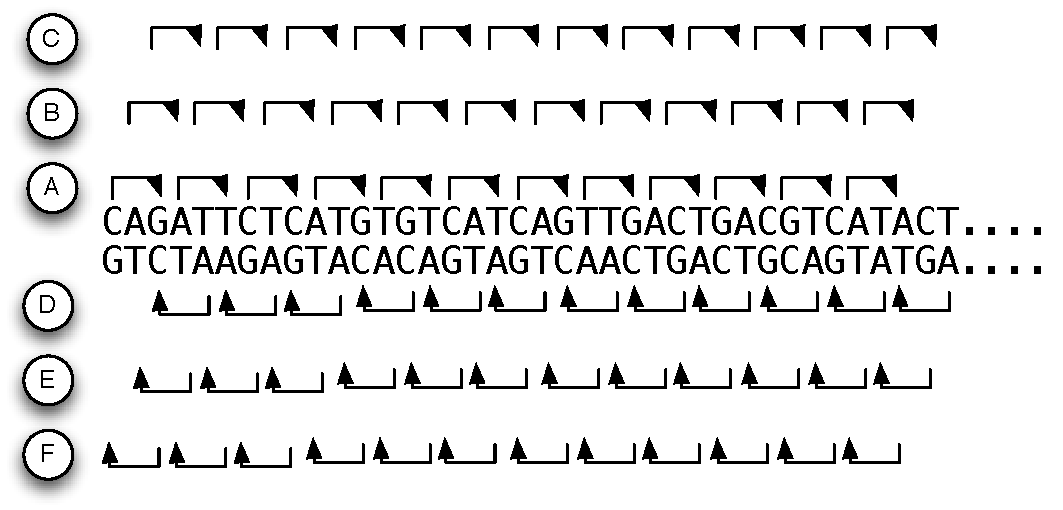
\includegraphics[width=0.7\textwidth]{reading_frame.pdf}
	\caption{Six possible reading frames.}
	\label{fig:gene_distribution_rib}
\end{figure}

So, to convert a base pair sequence (e.g. \texttt{CAGATTCTC}...) to a amino acid sequence (e.g. \texttt{GWLPHLQRI}...) you cut the base pair sequence in pieces of 3 nucleotides (e.g. \texttt{``CAG'', ``ATT'',...}), and use a conversion table that links any possible 3-mer to one of the 21 amnio acids. For instance, \texttt{CAG} codes for glutamine.

\subsection{All 3-mers}
To build the conversion table that links 3-mers to amino acids. We first need to build an exhaustive list of 3-mers. Write the code that takes as input the list of the four base pairs and generates as output all the possible permutations of size three.
	
The output should start like this and have 64 elements:
	
\begin{verbatim}
bases = ["t", "c", "a", "g"]
codons = ['ttt', 'ttc', 'tta', 'ttg', 'tct', 'tcc', 'tca', 'tcg', 'tat', ... ]
\end{verbatim}

\subsection{3-mer to amino acid}
We can now build a dictionary that links every 3mer to an amino acid. If you built the list in the same order as me in the previous step, the corresponding amino acids are the following:

\begin{verbatim}
aminos = "FFLLSSSSYY**CC*WLLLLPPPPHHQQRRRRIIIMTTTTNNKKSSRRVVVVAAAADDEEGGGG"
codon_to_amino = {'aaa': 'K', 'aac': 'N', 'aag': 'K', 'aat': 'N', 'aca': 'T', ... }
\end{verbatim}

\subsection{Sequence to protein}
You can now write the function that takes a nucleotide sequence as entry and outputs a protein sequence.

\begin{quote}
\begin{verbatim}
	def seq_to_prot(seq): ...........
\end{verbatim}
\end{quote}

You should be able to use it like this:
\begin{quote}
\begin{verbatim}
	seq_to_prot('cagattctc')
	>>> QIL
\end{verbatim}
\end{quote}

\subsection{Testing the three reading frames}
You can now load the file \texttt{"sequence\_001.txt"} and call the function you wrote in the last step with the six different possible frames and decide which one is right one.


\section{BLAST}
A common use of the BLAST tool is to identify the function of an unknown sequence. You have been provided with the sequence of a DNA fragment, \texttt{"fragment\_007.fasta"} from an unknown micro-organism. Your aim is to use the NCBI BLAST programs to determine what kind of protein is \texttt{fragment\_007} is likely to encode.\\

\url{http://blast.ncbi.nlm.nih.gov/Blast.cgi}

\subsection{Nucleotide BLAST - blastn}
Perform a nucleotide BLAST using \texttt{fragment\_007.fasta} 
\begin{enumerate}
\item Do you get any matches to \texttt{fragment\_007}? Which parameters did you use? Record the alignment statistics for the top hits.

\item Extract the sequence of the hit with the highest query coverage (this may not necessarily be the top hit) and perform another nucleotide BLAST, using the same parameters. Record the alignment statistics for the top hits.

\item What changes do you observe in the E-values? To which parameter would you attribute the these changes?  

\item What is the default threshold for the E-value on NCBI BLAST?

\item Do you have any significant hits suggesting a possible function for \texttt{fragment\_007}? 
\end{enumerate}

\subsection{Protein BLAST - blastp}

Using the python function from the previous exercise, obtain the amino acid sequences for \texttt{fragment\_007.fasta} in three reading frames. Choose the appropriate reading frame and save the corresponding amino acid sequence in \texttt{aa\_007.fasta} format.\\

Perform a protein BLAST with \texttt{aa\_007.fasta} 

\begin{enumerate}
\item Are any well-known protein domains found? 

\item Do you get any significant hits? Record the alignment statistics for the top hits. 

\item What is the possible function of the protein encoded by \texttt{fragment\_007}?

\item Which species is most predominant in your BLAST output?

\item Is there a BLAST program that would have given you the same results as BLASTp using the nucleotide sequence of \texttt{fragment\_007} as input?

\item How do results from BLASTp compare with the results from BLASTn?

\end{enumerate}

\subsection{Finding orthologs}

You have been provided with the sequence of the Pho2p protein from the famous yeast, \emph{Saccharomyces cerevisiae}. Run BLAST to find out whether any putative orthologs of Pho2p are present in another, not so famous yeast, \emph{Candida glabrata}.\\

In a paper comparing the phosphate signal transduction in \emph{S. cerevisiae} and \emph{C. gabrata} (Genetics 182:471-9,2009), the authors identified the ortholog of Pho2p in \emph{C. gabrata}. \\

Are the findings of the paper consistent with your observations?

\section{Some BLAST tips}

\begin{enumerate}
\item This web page provides useful guidelines for BLAST usage and explains the different flavors of BLAST:
\url{http://www.clcbio.com/index.php?id=995}

\item \emph{Reciprocal Best Hit}

This is a simple and commonly used test for predicting orthologous sequences.

Genes A (from species X) and B (from species Y) will be considered as (putative) orthologs if (1) a search of similar sequences of A in species Y yields as the best hit B, AND a search of similar sequences of B in species X yields as the best hit A.
\end{enumerate}

\end{document}
